% WIP-Stil LaTeX-Vorlage für (englischsprachige) Abschluss- und Studienarbeiten

\documentclass[
	11pt,								% Schriftgroesse
	DIV10,								% Koma-Script-Klassen: Groesse des bedruckbaren Bereichs
	a4paper,         					% Format
	oneside,							% Einseitiges Dokument
	headheight=20pt,					% Höhe Dokumentenkopf
	footheight=20pt,					% Höhe Dokumentenfuß
    parskip=full,						% Abstand zwischen Absaetzen (ganze Zeile)
    listof=totoc,						% Verzeichnisse im Inhaltsverzeichnis aufführen
	bibliography=totoc,					% Literaturverzeichnis im Inhaltsverzeichnis aufführen
	index=totoc,						% Index im Inhaltsverzeichnis aufführen
	%final
    %draft								% Status des Dokuments
]{scrartcl}

%%% Schrift %%%
\usepackage[utf8]{inputenc}				% Umlaute im Tex-Code erlauben
\usepackage[T1]{fontenc}
\usepackage[ngerman, english]{babel}	% Sprachpaket Deutsch
\usepackage[useregional]{datetime2}
\selectlanguage{english}
\usepackage{csquotes}					% Zitation im gleichen Stil 
\renewcommand{\baselinestretch}{1.50}	% Zeilenabstand 1.5
\normalsize
%\usepackage{uarial}						% Schriftart Arial, kann ausdokumentiert werden, wenn die Standardschrift benutzt werden soll
\renewcommand{\familydefault}{\sfdefault}
\usepackage{blindtext}					% zum Testen des Layouts
\usepackage{microtype}					% Verbesserter Randausgleich
\usepackage{color}
\usepackage{eurosym} 					% Eurozeichen
\usepackage{xcolor}
\usepackage{datetime}
\usepackage{dcolumn}

%%% Anpassung des Formats %%%
\RedeclareSectionCommand[
  beforeskip=-1sp,						% minimaler Abstand nach Überschrift, anschließend nicht einrücken
  afterskip=1sp]{section}
\RedeclareSectionCommand[
  beforeskip=-1sp,						% siehe oben 
  afterskip=1sp]{subsection}
\RedeclareSectionCommand[
 beforeskip=-1sp,						% siehe oben
  afterskip=1sp]{subsubsection}
\RedeclareSectionCommand[
  beforeskip=-1sp,						% siehe oben
  afterskip=1sp]{paragraph}
\RedeclareSectionCommand[
 beforeskip=-1sp,						% siehe oben
 afterskip=1sp]{subparagraph}

%%% Änderungen des Inhaltsverzeichnis %%%
\usepackage[titles]{tocloft}			% wird zur Änderung des toc verwendet

\renewcommand{\cftsecleader}			% führe Punkte im toc auch für sections ein, Punkte fetter als normal
	{\bfseries\cftdotfill{\cftdotsep}}
\renewcommand{\cftdotsep}{0.1}			% setze Punkteabstand enger	

%%% definiere Inhaltsübersicht %%%
% Achtung: In Vorlage auskommentiert %
\newcommand*\inhaltsuebersicht{%
\section*{Content Overview}				% Name 
\begingroup
\value{tocdepth}\shorttocdepth\relax
\makeatletter
\input{\jobname.toc}
\makeatother
\endgroup
}
\newcommand*{\shorttocdepth}{1}			% Tiefe der Inhaltsübersicht == 2

%%% Bilder %%%
\usepackage{graphicx}
\graphicspath{{./Bilder/}}				% Bilderverzeichnis
\usepackage{overpic} 					% Beschriftung in Abbildung platzieren
\usepackage{here}						% Bildplatzierung mit [H]

%%% Verschiedenes, Mathe-Funktionen, Layout %%%
\usepackage{float,caption}
\usepackage{amsmath,amsfonts}
\usepackage{mathtools}
\usepackage{amssymb}
\usepackage{exscale}
\usepackage[normalem]{ulem}
\usepackage{setspace}
\usepackage[a4paper,
    lmargin={2.5cm},
    rmargin={2.5cm},
    tmargin={2cm},
    bmargin={2cm}
    ]{geometry}
    
\addtolength{\footskip}{-0.5cm}			% Fussbereich 0.5cm höher, sodass die Seitennummierung höher ist

%%% Listen %%%
%\usepackage{enumitem}
\usepackage{paralist}					% Für kompakte Listen
\setlength{\pltopsep}{5pt}				% setzt den oberen Abstand der compactitem- und compactenum-Liste auf eine Zeilenbreite

%%% Tabellen %%%
\usepackage{tabularx}
\usepackage{booktabs}					% Platzverschwendung in Tabellen vermeiden
\usepackage{array}						% mehr Möglichkeiten der Darstellung

%%% Kopf und Fußzeile %%%
\usepackage[nouppercase,headsepline]{scrpage2}
\pagestyle{scrheadings}
\clearscrheadfoot
%\chead{\textit{TU Berlin, Fachgebiet Wirtschafts- und Infrastrukturpolitik (WIP)}}
	% Leerzeichen zwischen FN-Nummer und FN-Text
\deffootnote[]{1.5em}{1em}{\textsuperscript{\thefootnotemark}\enskip}
\cfoot{\normalsize{\emph{\thepage}}}

%%% URL's %%%
\usepackage[lowtilde]{url}				% bei Verwendung eines Tildezeichens wird es normal gesetzt
\urlstyle{same}
\usepackage{etoolbox}

%%% Zitation %%%
\usepackage[style=chicago-authordate,
			%style=authoryear,
            giveninits,					% Vornamen abkürzen
			maxbibnames=10,				% in der Bib werden 10 Autoren ausgegeben (bis zu 10)
            maxcitenames=2,				% max. 3 Autoren bei \cite
            backend=biber,
			doi=false,
			isbn=false,
			url=false,
            natbib=true,				% verwendet Natbib 
            sorting=nyt					
			]{biblatex}

\addbibresource{literatur.bib}
\usepackage{breakcites}

\DeclareNameAlias{author}{last-first}				

% *****************************************
%%% Anpassungen für englische Literatur %%%
% *****************************************

\DeclareFieldFormat[article]{title}{"#1\adddot"}				
\DeclareFieldFormat[inproceedings]{title}{"#1\addcomma"}				
%\DeclareFieldFormat[book]{title}\textit{{#1}\isdot}    			
\DeclareFieldFormat[techreport]{title}{"#1\adddot"}					
\DeclareFieldFormat[incollection]{title}{"#1\adddot"} 
\DeclareFieldFormat[online]{title}{#1\isdot}           		
\DeclareFieldFormat[misc]{title}{"#1\isdot"}					

\DeclareFieldFormat[inproceedings]{booktitle}{proceedings of #1}	

\AtEveryBibitem{\clearlist{language}}

\AtEveryBibitem{%
	\ifentrytype{online}
	{}
	{\clearfield{urlyear}\clearfield{urlmonth}\clearfield{urlday}}}

\AtEveryBibitem{%
	{\clearfield{month}\clearfield{day}}}

\DefineBibliographyStrings{english}{andothers = {et\,al\adddot}}

\DeclareFieldFormat[article]{number}{#1}					
\DeclareFieldFormat[article]{pages}{\space#1}

\usepackage{xpatch}
\xpretobibmacro{author}{\mkbibbold\bgroup}{}{}					% Autor fett
\xapptobibmacro{author}{\egroup}{}{}

\DeclareSourcemap{
	\maps{\map{
			\step[fieldsource=language, fieldset=langid, origfieldval, final]
			\step[fieldset=language, null]}}}

\usepackage[pdfborder={0 0 0},								% Rahmen in pdf nicht sichtbar
			breaklinks=true,
            %draft,											% alle Links abschalten
            ]{hyperref}

%%%%%%%%%%%%%%%%%%%%%%%%%%%%%%%%%%%%%%%%%%%%%%%%%%%%%%%%%%%%%%%%%%%%%%%%%%%%%%%%%%%%%%%%%%%%%%%
% Beginn des Dokument

% *************************************
%%% HIER DIE TITELSEITE BEARBEITEN %%%%
% *************************************

%%% Titelseite %%%
\newcommand{\autor}{Author 1} 		% Name des Autors
\newcommand{\matriculation}{xxxxxx} 
\newcommand{\mailaddress}{xxxxx@campus.tu-berlin.de}
\newcommand{\autorzwei}{Author 2}
\newcommand{\matriculationzwei}{xxxxxx} 
\newcommand{\mailaddresszwei}{xxxxx@campus.tu-berlin.de}
\newcommand{\autordrei}{Author 3}
\newcommand{\matriculationdrei}{xxxxxx} 
\newcommand{\mailaddressdrei}{xxxxx@campus.tu-berlin.de}

\newcommand{\betreuer}{Prof. Dr. Christian von Hirschhausen} 		% Namen der Betreuer
\newcommand{\betreuerzwei}{Second supervisor}
                      
                  
%\newcommand{\datum}{\selectlanguage{ngerman}\today}
\newcommand{\engdate}{\selectlanguage{english}April 20, 2018}

%%% Glossar und Abkürzungsverzeichnis %%% 
\usepackage[acronym,
            nonumberlist,									% keine Seitenzahlen anführen
            toc,											% im Inhaltsverz. mit aufnehmen
            style=super,									% Einträge mit Abstand setzten 
            nopostdot,										% kein schließender Punkt
           	nogroupskip]									% kein Absatz zwischen Gruppen
           	{glossaries}									% muss nach \usepackage{hyperref} geladen werden, damit auch Einträge des Abkürzungsverzeichnisses verlinkt sind
\makeglossaries

%***********************************
%%% HIER DIE AKRONYME DEFINIEREN %%%
%***********************************

%%% exempl. Akronyme %%%
\newacronym[firstplural=renewable energy sources (RES)]{res}{RES}{renewable energy sources}
\newacronym{eeg}{EEG}{Erneuerbare-Energien-Gesetz}
\newacronym{tso}{TSO}{Transmission System Operator}
\newacronym{rmse}{RMSE}{root-mean squared error}
\newacronym{gams}{GAMS}{General Algebraic Modeling System}
\newacronym[firstplural=Energiewirtschaftsgesetzes (EnWG)]{enwg}{EnWG}{Energiewirtschaftsgesetz}
\newacronym{ihv}{i.H.v.}{in Höhe von}
\newacronym[firstplural=Millimetern (mm)]{mm}{mm}{Millimeter}
\newacronym[firstplural=Off\-shore-Wind\-parks (OWP)]{owp}{OWP}{Off\-shore-Wind\-park}
	% sort= ermöglicht korrekte Sortierung von Umlauten
\newacronym[sort=uebertr]{unb}{\"UNB}{Übertragungsnetzbetreiber}

% ***********************************************************************************
% Beginn des Dokuments
% ***********************************************************************************

\begin{document}\selectlanguage{english}
% ***********************************************************************************
% Automatische Zusammensetzung der Titelseite, nur aendern, falls noetig!
% ***********************************************************************************

	\thispagestyle{plain}
	\begin{titlepage}
		\vspace{0cm} 
		\begin{center}
			
\includegraphics[width=2.5cm]{pictures/TU_Logo_kurz_4c_rot}\\
			\normalsize{Technische Universität Berlin}\\
			Fakultät VII Wirtschaft \& Management\\
			Fachgebiet Wirtschafts- und Infrastrukturpolitik (WIP)
		\end{center}
        \vfill
		%\vspace*{\fill}
		\begin{center}
			%\Large{\textbf{\textsc{\doctitle}}}\\
			\Large{\textbf{Course}}\\
            \LARGE{\textbf{Title}}\\[2ex]
            \Large{\textbf{Subtitle}}
            
			\vfill
			
% "Ockerfarbener Kasten":

%{
%\setlength{\fboxrule}{0.2mm}
%\definecolor{ocker}{RGB}{196,188,150}
%			\selectlanguage{ngerman}\normalsize
%\fcolorbox{black}{ocker}{\begin{minipage}{\textwidth}

%\textbf{Dateinamen-Kern (mit Versions-Nr. 000):} 
%\url{vorlage_latex_v000}

%\textbf{Ablage-Server-Pfad (fixiert):} 
%\url{Z:\\lehre\\BEREICH_WIPOL_ETC\\veranstaltung___ewa_seminar\\_formatvorlagen\\LaTeX-Vorlagen\\Standard}

%\textbf{Aktueller Ablageort:} \url{\\\\afs\\tu-berlin.de\\units\\Fak_VII\\wip\\share\\lehre\\BEREICH_WIPOL_ETC\\veranstaltung___ewa_seminar\\_formatvorlagen\\LaTeX-Vorlagen\\Standard\\vorlage_latex_v001_vc_17-05-2017}

%\textbf{Datum:} \today \ \currenttime
%\end{minipage}}}

			\vfill
			\normalsize
			Author(s): \\
			\autor \, (\matriculation) - \mailaddress \\
			\autorzwei \, (\matriculation) - \mailaddress \\
			\autordrei \, (\matriculation) - \mailaddress \\
            \vfill
			Supervisors:\\\betreuer	\\
			\betreuerzwei
			%\vspace*{\fill}
            \vfill
			Berlin, \engdate
		\end{center}
		
	\end{titlepage}
	\newpage
	\pagenumbering{roman}
	
% ***********************************************************************************
% Eidesstattliche Erklaerung, automatisch generiert
% ***********************************************************************************


\setcounter{page}{2}							% Seitenzahl == 2 (Titelseite wird mitgezählt)
% \chead{\textit{Eidesstattliche Erklärung}}
% \section*{Eidesstattliche Erklärung}
%	
%	Hiermit erkläre ich, \autor, an Eides statt, dass ich die vorliegende Arbeit selbstständig und nur unter Zuhilfenahme der ausgewiesenen Hilfsmittel angefertigt habe.\\
%	Sämtliche Stellen der Arbeit, die im Wortlaut oder dem Sinn nach anderen gedruckten oder im Internet verfügbaren Werken entnommen sind, wurden durch genaue Quellenangaben kenntlich gemacht.
%
%	

\chead{\textit{Statutory declaration}}
\section*{Statutory declaration}
	Hereby, I declare that I have developed and written this research completely by myself and that we have not used sources or means without declaration in the text. Any external thought, content, media, or literal quotation is explicitly marked and attributed to its respective owner or author. \\
	As of the date of submission, this piece of doument and its content have not been submitted anywhere else but to our supervisors.
	
	\bigskip
	
	Berlin, \engdate
	
	\bigskip
	\bigskip
		\begin{center}	
			\begin{minipage}[t]{0.3\textwidth}
				\rule[-0.2cm]{4.5cm}{0.5pt} \\
				\textsc{\autor}
			\end{minipage}
			\begin{minipage}[t]{0.3\textwidth}
				\rule[-0.2cm]{4.5cm}{0.5pt} \\
				\textsc{\autorzwei}
			\end{minipage}
			\begin{minipage}[t]{0.3\textwidth}
				\rule[-0.2cm]{4.5cm}{0.5pt} \\
				\textsc{\autordrei}
			\end{minipage}
		\end{center}
	
	\newpage

% ****************************	
% Abstract und ggf. Zusammenfassung
% ****************************

	\chead{\textit{Abstract}}
	\section*{Abstract}
	
	Lorem ipsum dolor sit amet, consetetur sadipscing elitr, sed diam nonumy eirmod tempor invidunt
	ut labore et dolore magna aliquyam erat, sed diam voluptua. At vero eos et accusam et justo
	duo dolores et ea rebum. Stet clita kasd gubergren, no sea takimata sanctus est Lorem ipsum
	dolor sit amet. \\
	Lorem ipsum dolor sit amet, consetetur sadipscing elitr, sed diam nonumy eirmod tempor invidunt
	ut labore et dolore magna aliquyam erat, sed diam voluptua. At vero eos et accusam et justo
	duo dolores et ea rebum. Stet clita kasd gubergren, no sea takimata sanctus est Lorem ipsum
	dolor sit amet.
	
	\newpage	

% ***********************************************************************************
% Verzeichnisse
% ***********************************************************************************
	\selectlanguage{english}	
	
	\chead{\textit{Index}}
	\setcounter{tocdepth}{4} 					% Tiefe des Inhaltsverzeichnisses
    \setcounter{secnumdepth}{4}					% Tiefe der gezählten Überschriften
	
    \begingroup									% verringere Abstände in der Inhaltsübersicht
	\parskip=0pt	
    \endgroup
    \newpage
    \begin{onehalfspace}
    \chead{\textit{Contents}}
    \tableofcontents 							% Inhaltsverzeichnis
	\end{onehalfspace}
	\newpage
	\setkomafont{captionlabel}{\bfseries}
	\setkomafont{caption}{\bfseries}			% Bild- und Tabellenbeschriftung fett
		
	% Vor der Zahl steht Figure im Verzeichnis
	\renewcommand{\cftfigpresnum}{Figure }
	\settowidth{\cftfignumwidth}{Figure 5\quad}  
	\listoffigures								% Abbildungsverzeichnis
	%\newpage
		
	% Vor der Zahl steht Table im Verzeichnis
	\renewcommand{\cfttabpresnum}{Table }
	\settowidth{\cfttabnumwidth}{Table 150\quad}
	\newpage
	\listoftables								% Tabellenverzeichnis
	% \newpage
	%
	% %Glossary/List of Acronyms
	% \printglossary								% Glossar
	% \newpage
	% \printglossary[type=\acronymtype,			% Akronyme und Abkuerzungen
    %				title={List of Acronyms}]
    \newpage
	\pagenumbering{arabic}						% beginne mit "normaler" Nummerierung
	
% ***********************************************************************************
% Beginn des eigenstaendigen Teils
% ***********************************************************************************
\selectlanguage{english}


\chead{\textit{Introduction}}					% definiere Kopfzeile
%\include{files/Introduction}					% include statt input ermöglicht Arbeit mit \includeonly{} und fügt Seitenumbruch vor section ein

\section{Introduction}
\textbf{WICHTIG:}
\begin{enumerate}
	\item Mehrmals kompilieren!
	\item Biber benutzen.
	\item Glossary (F9) ausführen. [Achtung: makeglossaries benötigt Perl]
	\item MikTeX regelmäßig updaten!
\end{enumerate}


\subsection{Subsection}
Acronyms: \gls{tso}; \gls{gams}

\subsubsection{Subsubsection}
Chicago (author-date) citation style is used.\\
In-text citation:
\citet{abrell_integrating_2015} employed...

Other forms of citation:
.... (see \citealt{birge_introduction_2011})

\newpage

\chead{\textit{Second chapter}}  			% definiere Kopfzeile
\section{Second chapter}

\subsection{Exemplary Table}\label{ex_table}
Please maintain a consistent table style (booktabs). For convenience, feel free to use a \href{https://www.tablesgenerator.com/}{TeX table generator}.
\begin{table}[H]
	\centering
	\caption{An exemplary table}
	\begin{tabular}{lll}
		\hline
		\textbf{First Column}		   & \textbf{Second Column}     & \textbf{Third Column}       \\ \hline
		First Row                      & information     			& information     \\
		Second Row                     & information     			& information     \\
		Third Row					   & information     			& information     \\ \hline
	\end{tabular}
\end{table}
\begin{flushleft}
	\quad\quad\footnotesize{Source: Based on \citet{leuthold_large-scale_2012}.}
\end{flushleft}


\subsection{Exemplary Figure}

\begin{figure}[H]
	\centering
	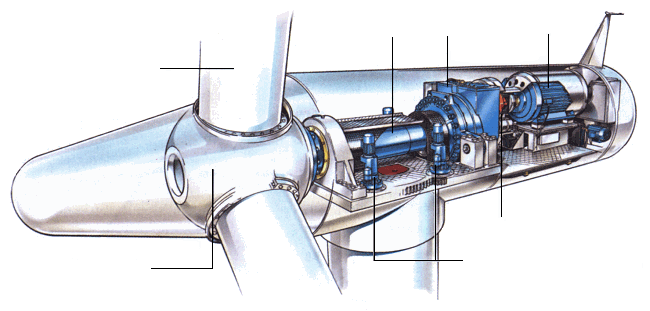
\includegraphics[width=\textwidth]{pictures/wind_turbine.png}
	\caption{An exemplary figure}
	\label{wind_turbine}
	\flushleft\quad\quad\footnotesize{Source: Own illustration.}
\end{figure}	

\newpage

% weitere Dokumente einfügen mit den gleichen zwei Befehlen

%\nocite{*}									% gibt zum Testen des Literaturverzeichnisses alle Bibeinträge aus
\chead{\textit{References}}				    % siehe oben 
\renewcommand\refname{References}			% in Literaturverzeichnis umbenennen
\printbibliography
%[heading=bibintoc]
\end{document}
